\section*{\centerline{Chords Overview}}
~\\~\\
%
\makebox[\textwidth][s]{\textit{~~dur ~~~~ 6 ~~~~ 7~~}}\\~\\~\\
%
\noindent\hfill
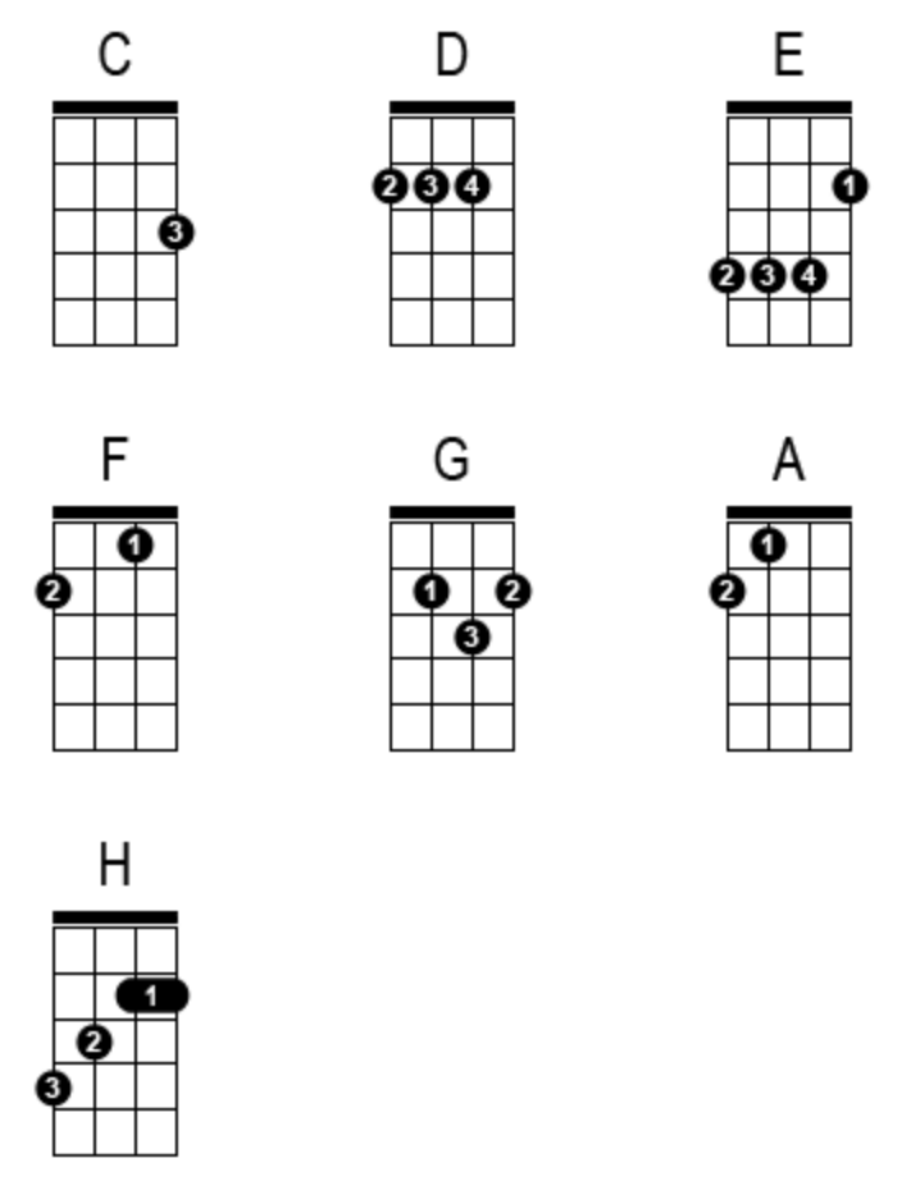
\includegraphics[width=0.25\linewidth]{../images/acc01_dur}
\hfill
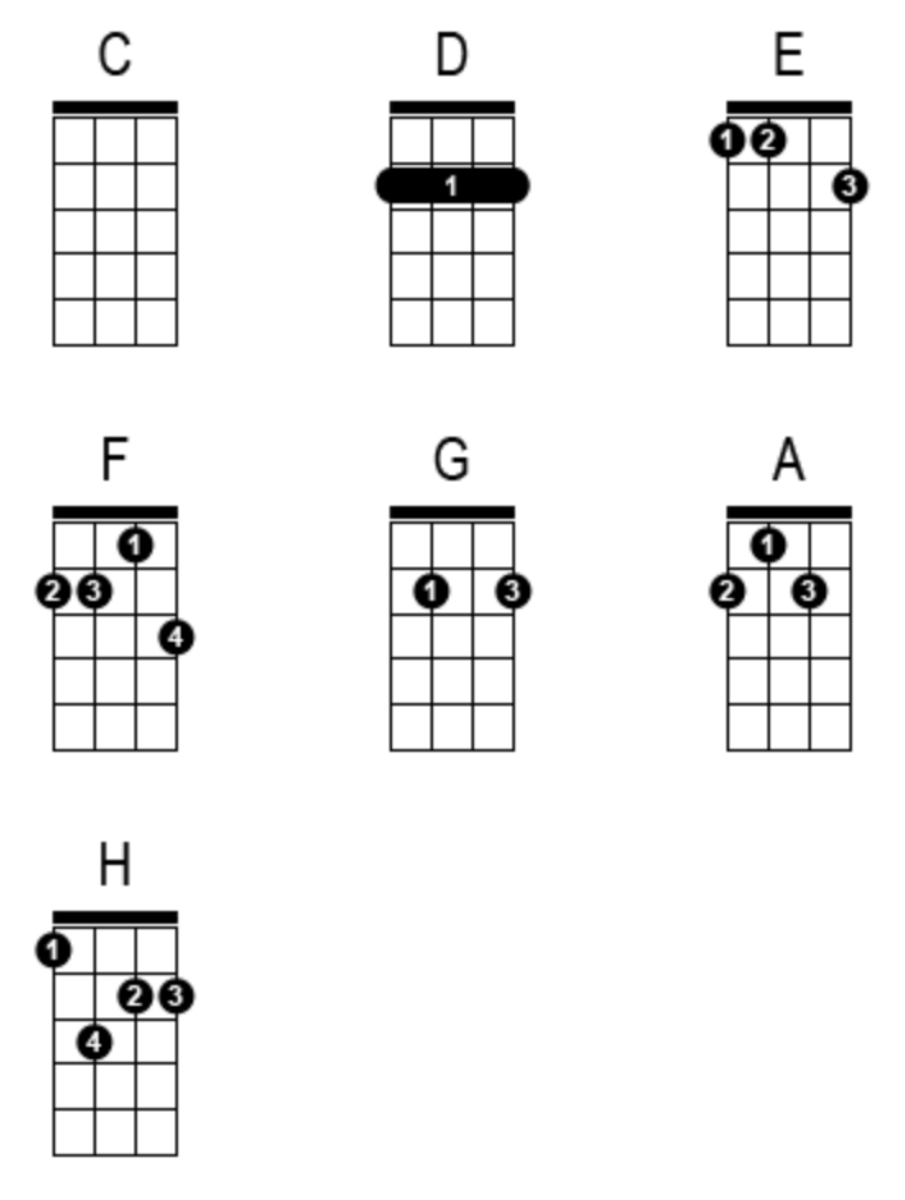
\includegraphics[width=0.25\linewidth]{../images/acc02_6}
\hfill
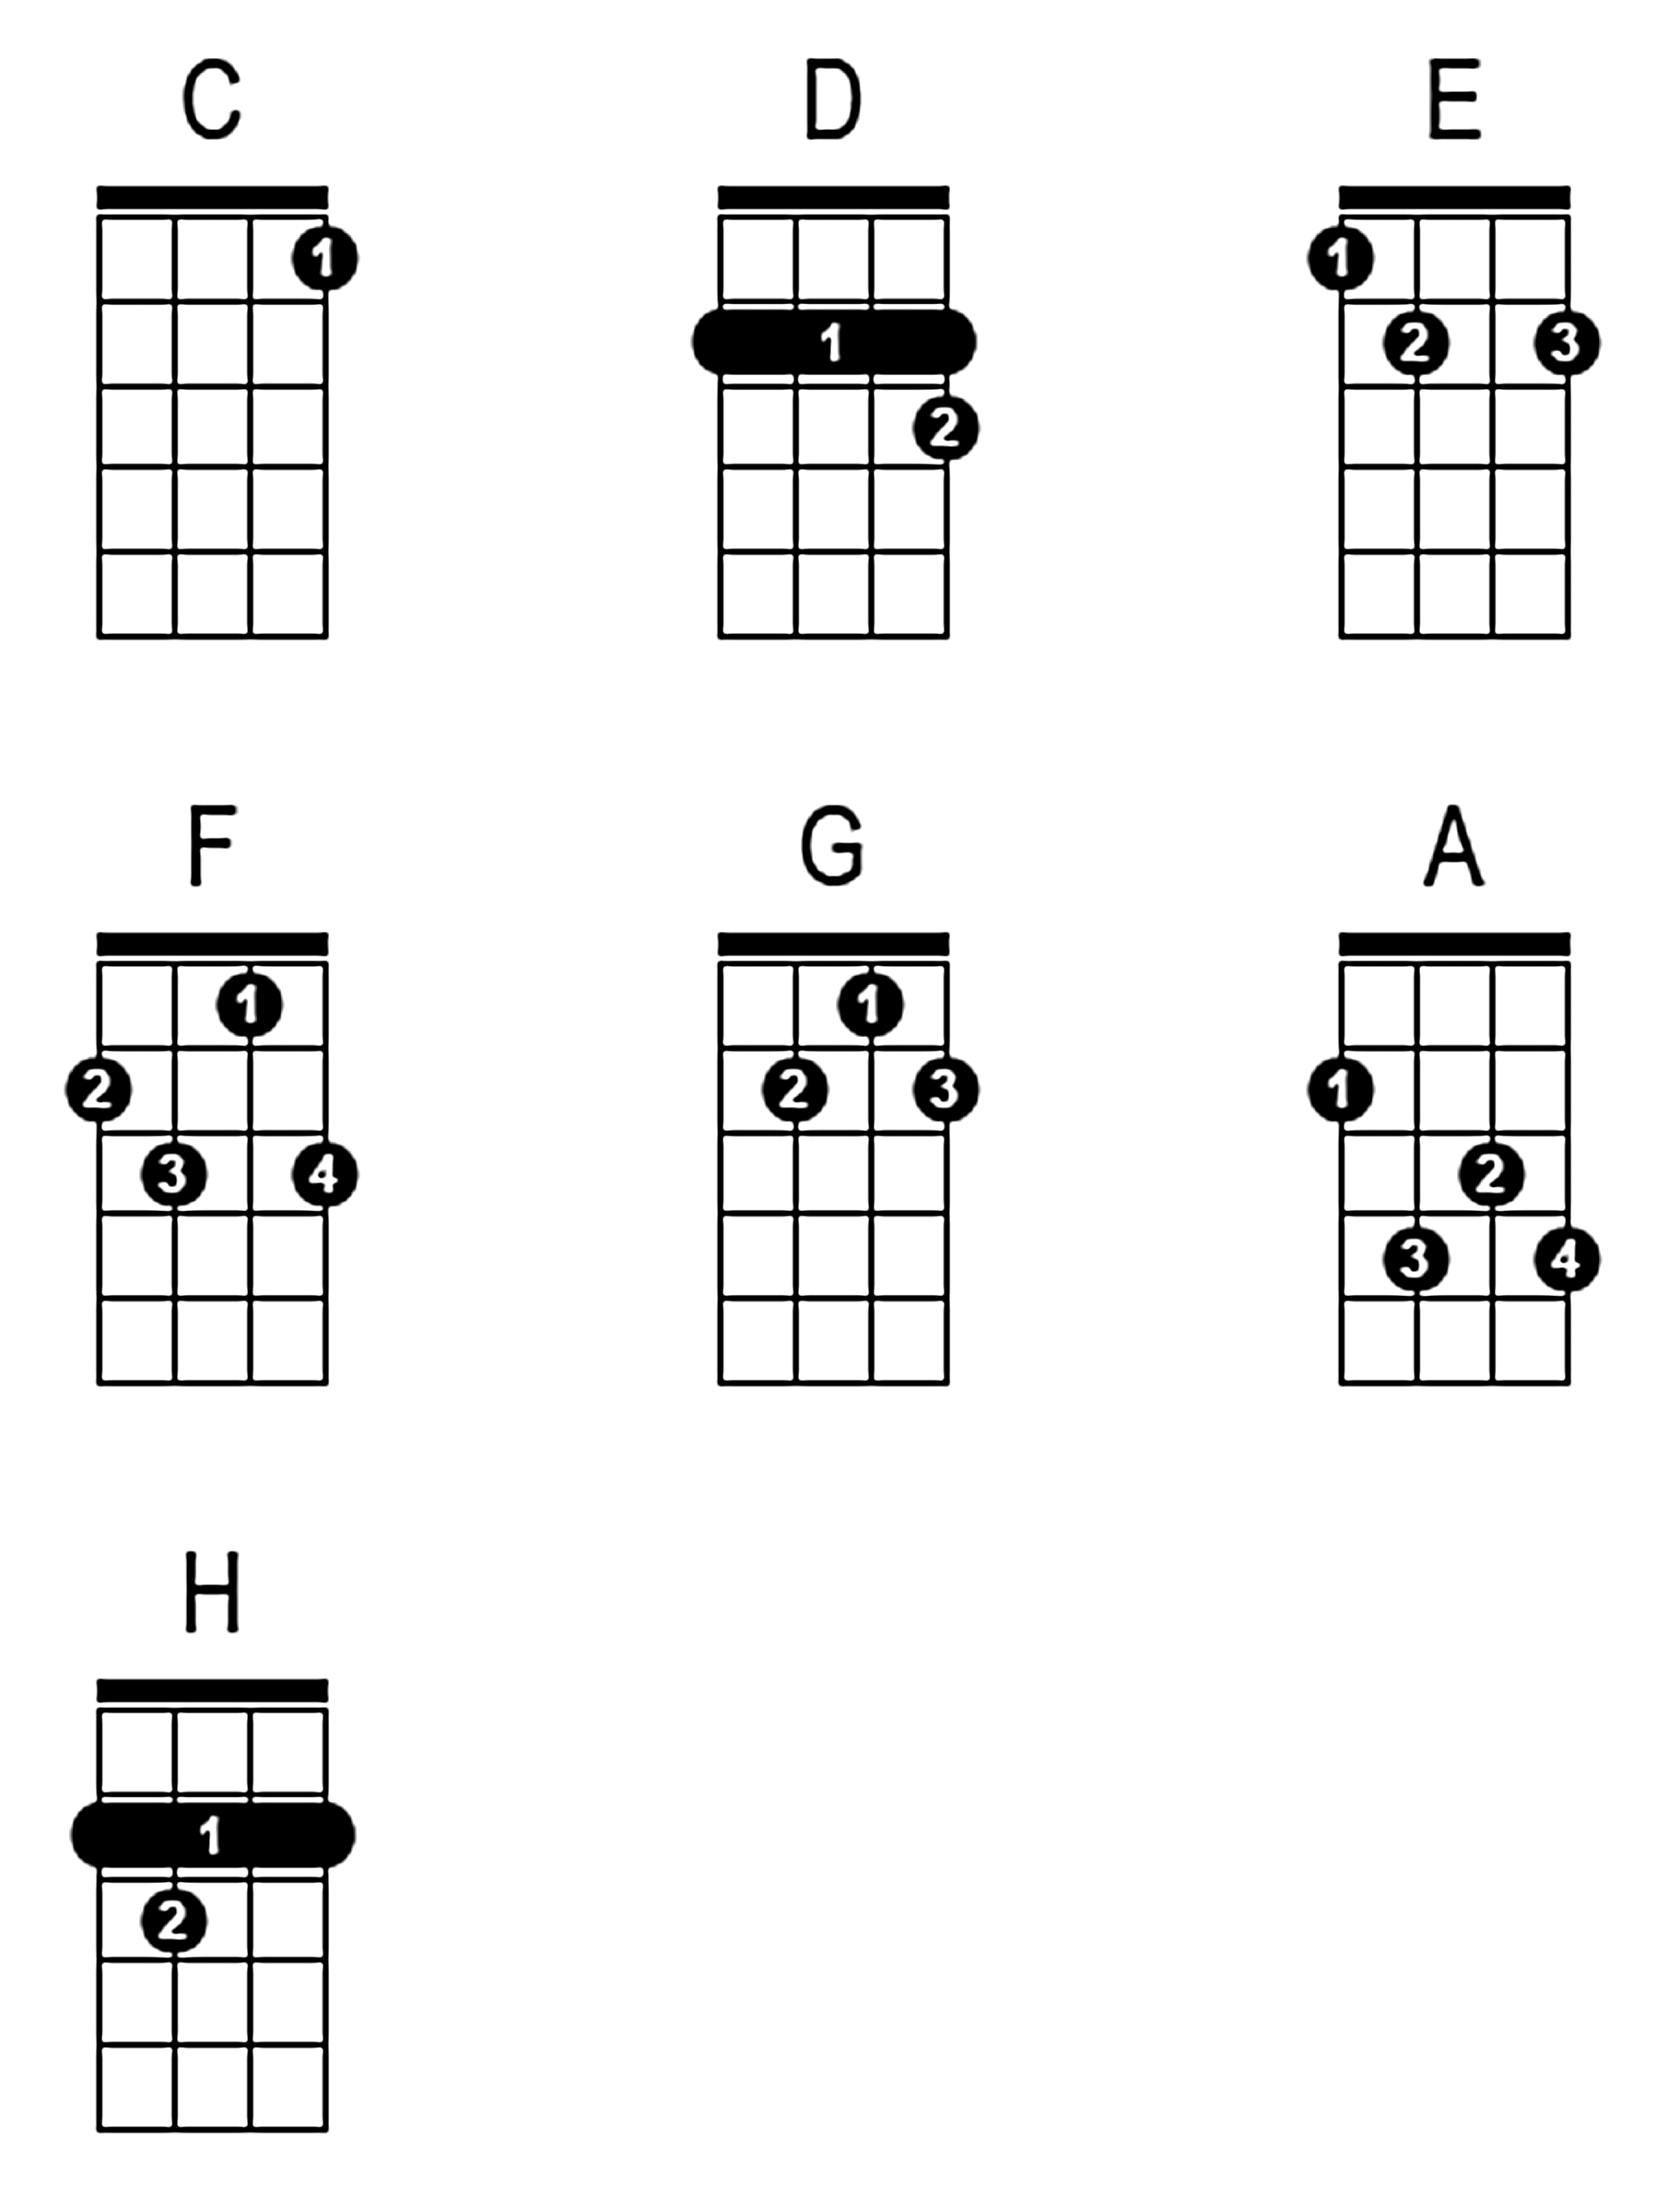
\includegraphics[width=0.25\linewidth]{../images/acc03_7}
\hfill\\
%
~\\~\\~\\~\\~\\
%
\makebox[\textwidth][s]{\textit{~~moll ~~~~ m6 ~~~~ m7~~}}\\~\\~\\
%
\noindent\hfill
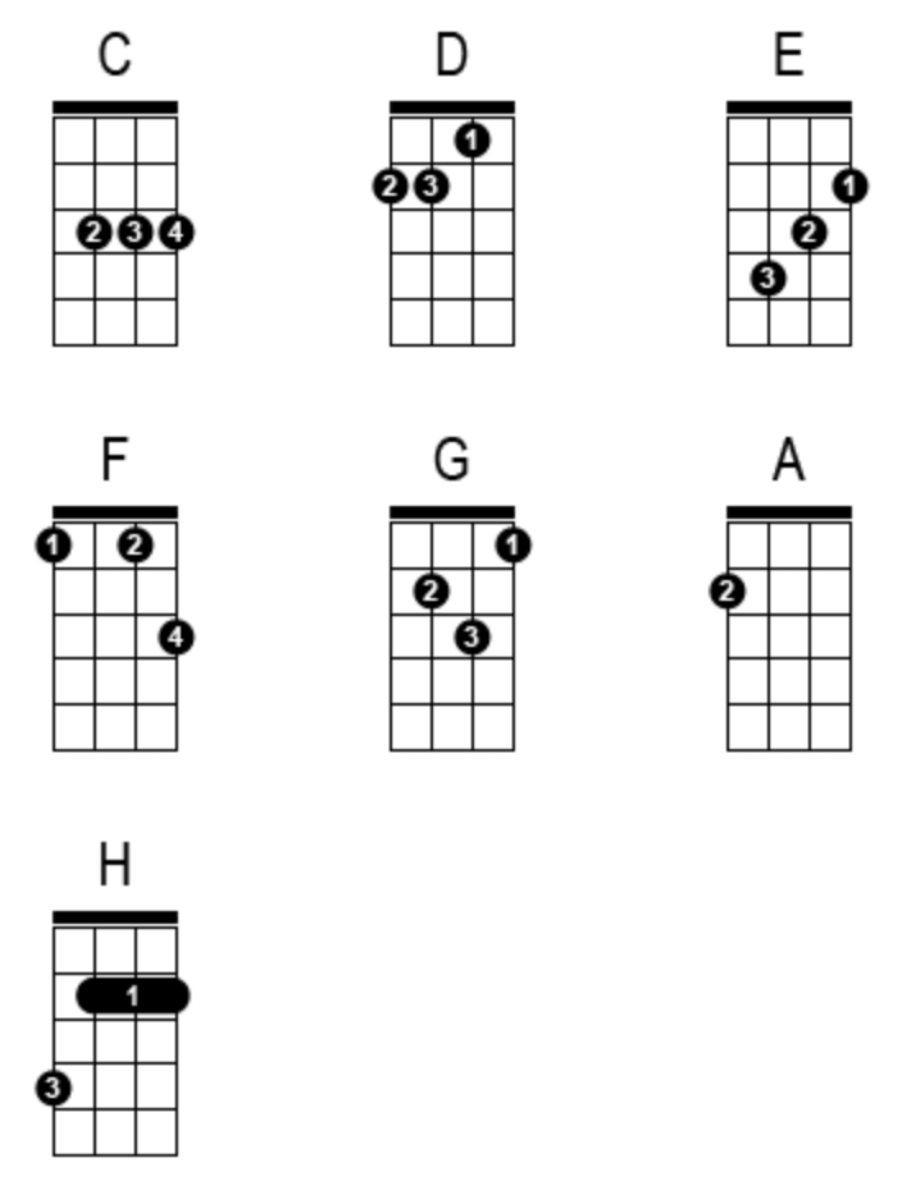
\includegraphics[width=0.25\linewidth]{../images/acc04_moll}
\hfill
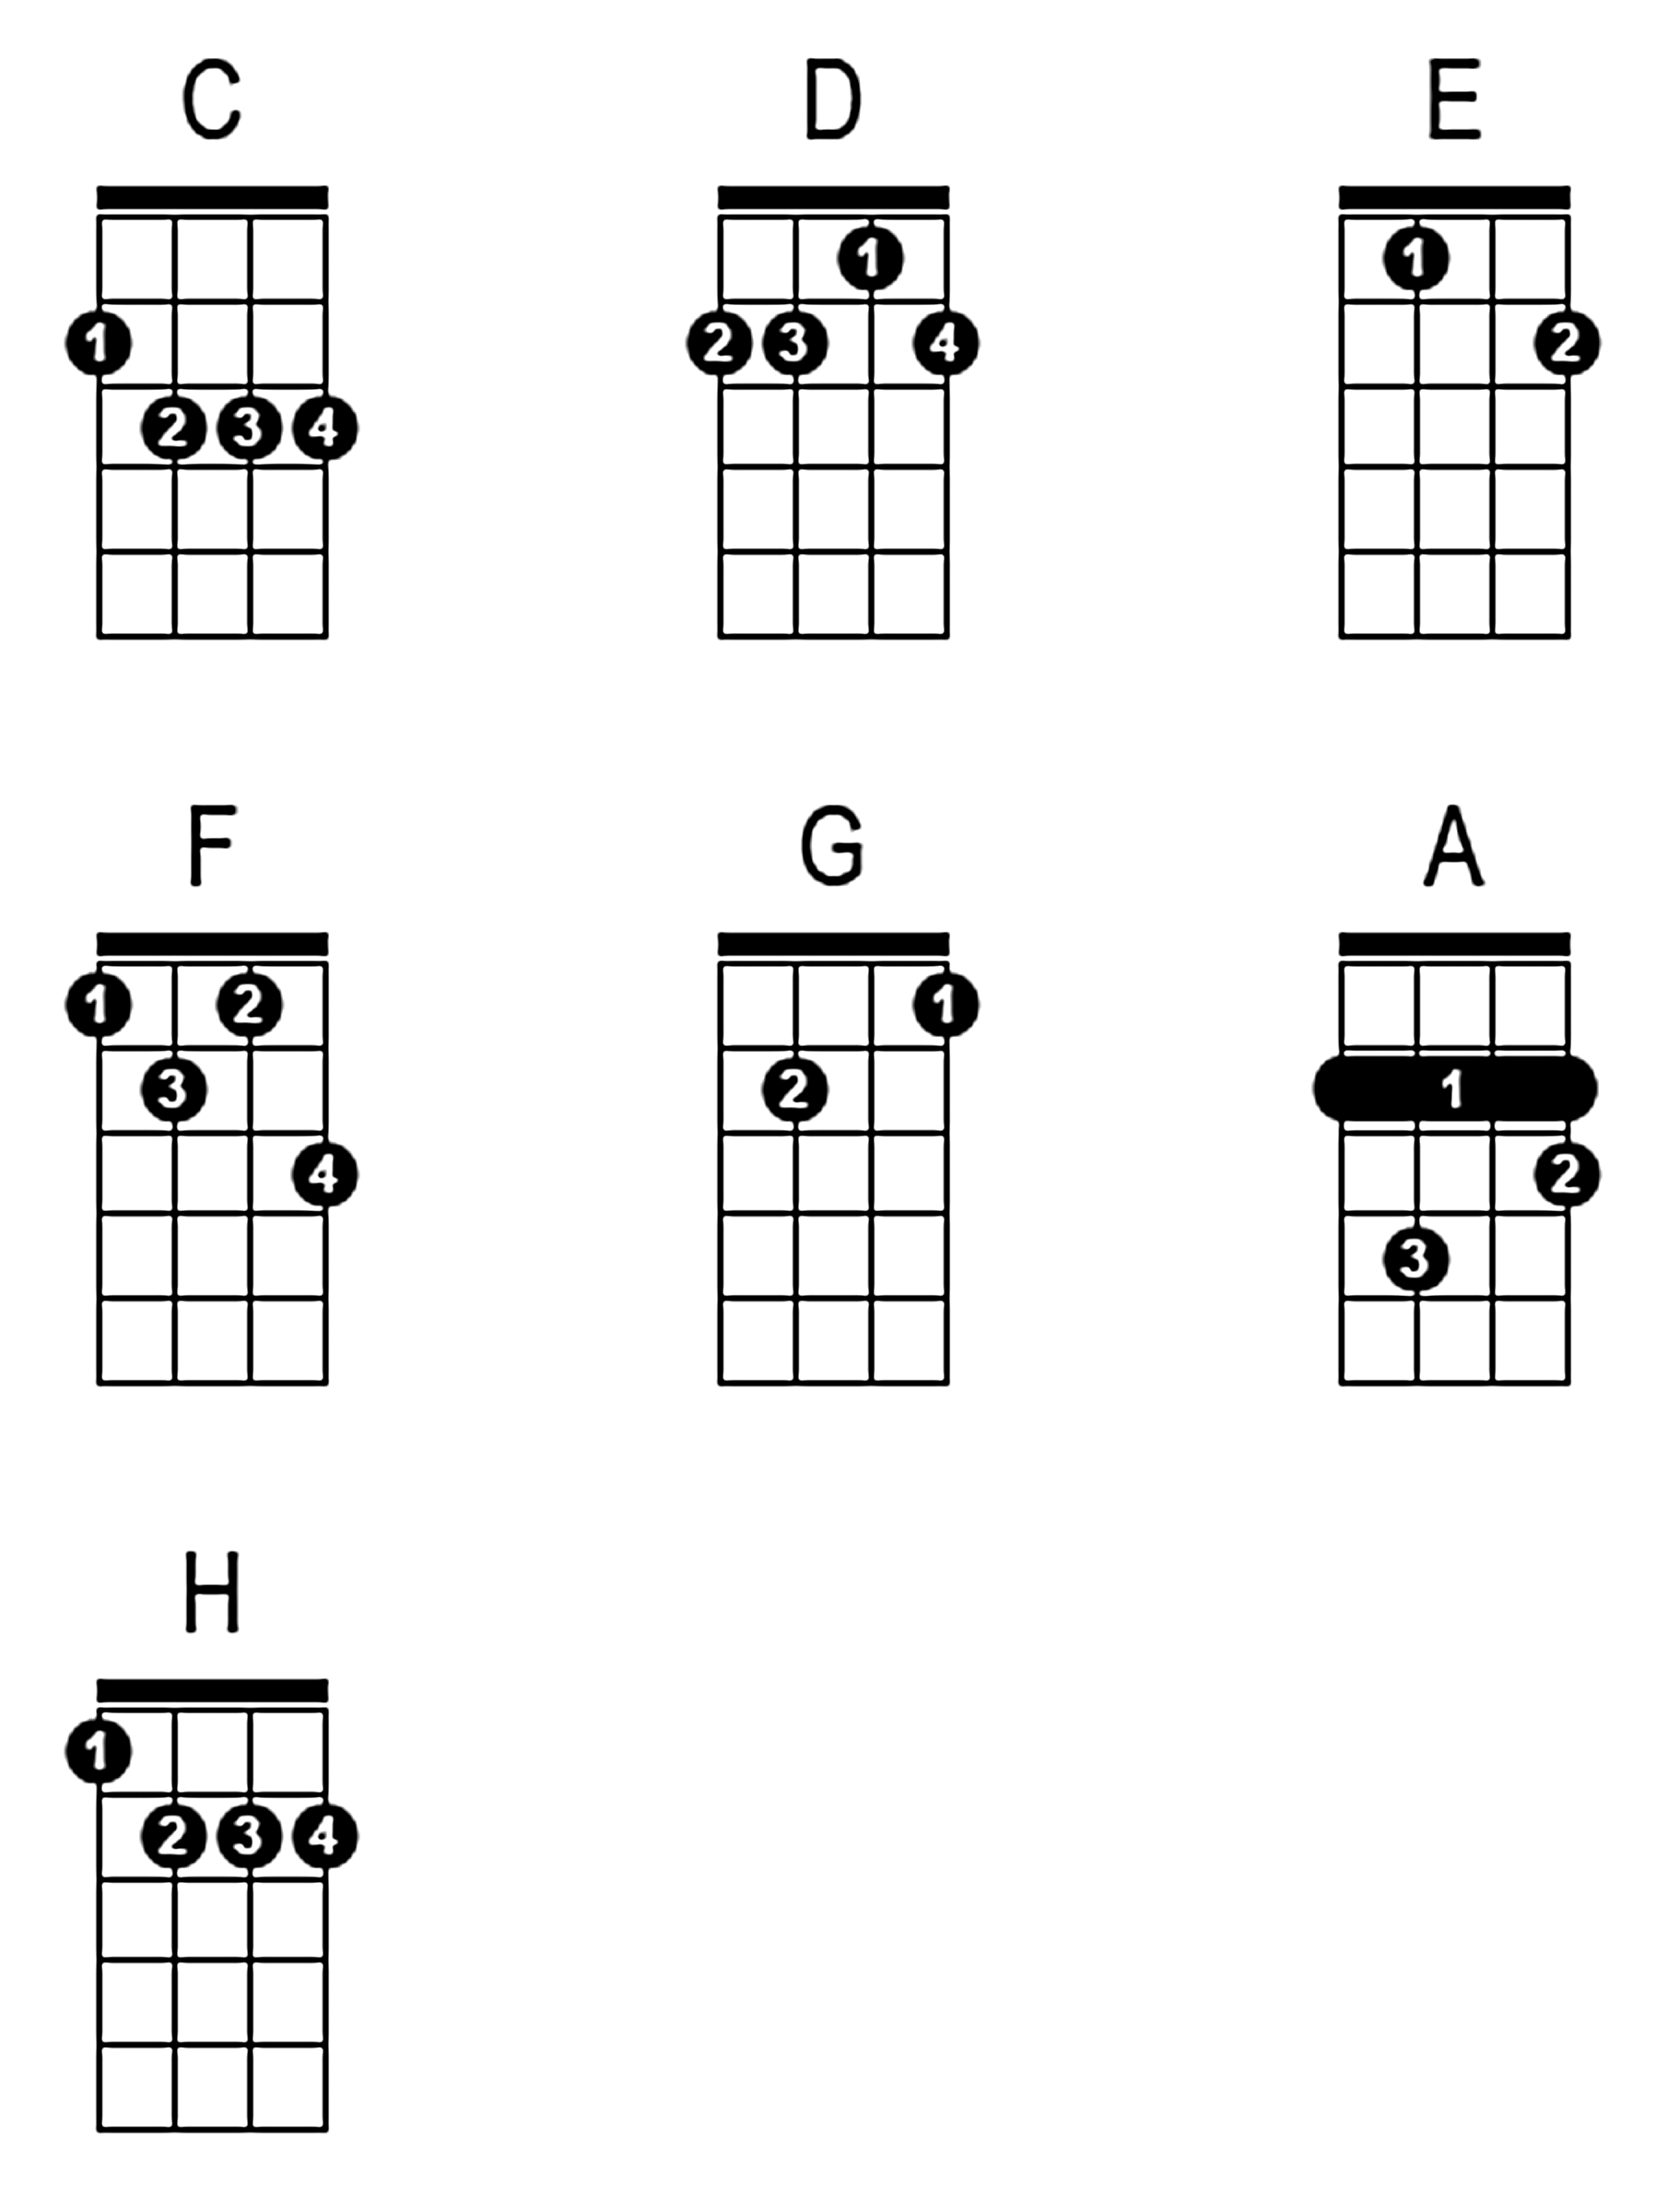
\includegraphics[width=0.25\linewidth]{../images/acc05_m6}
\hfill
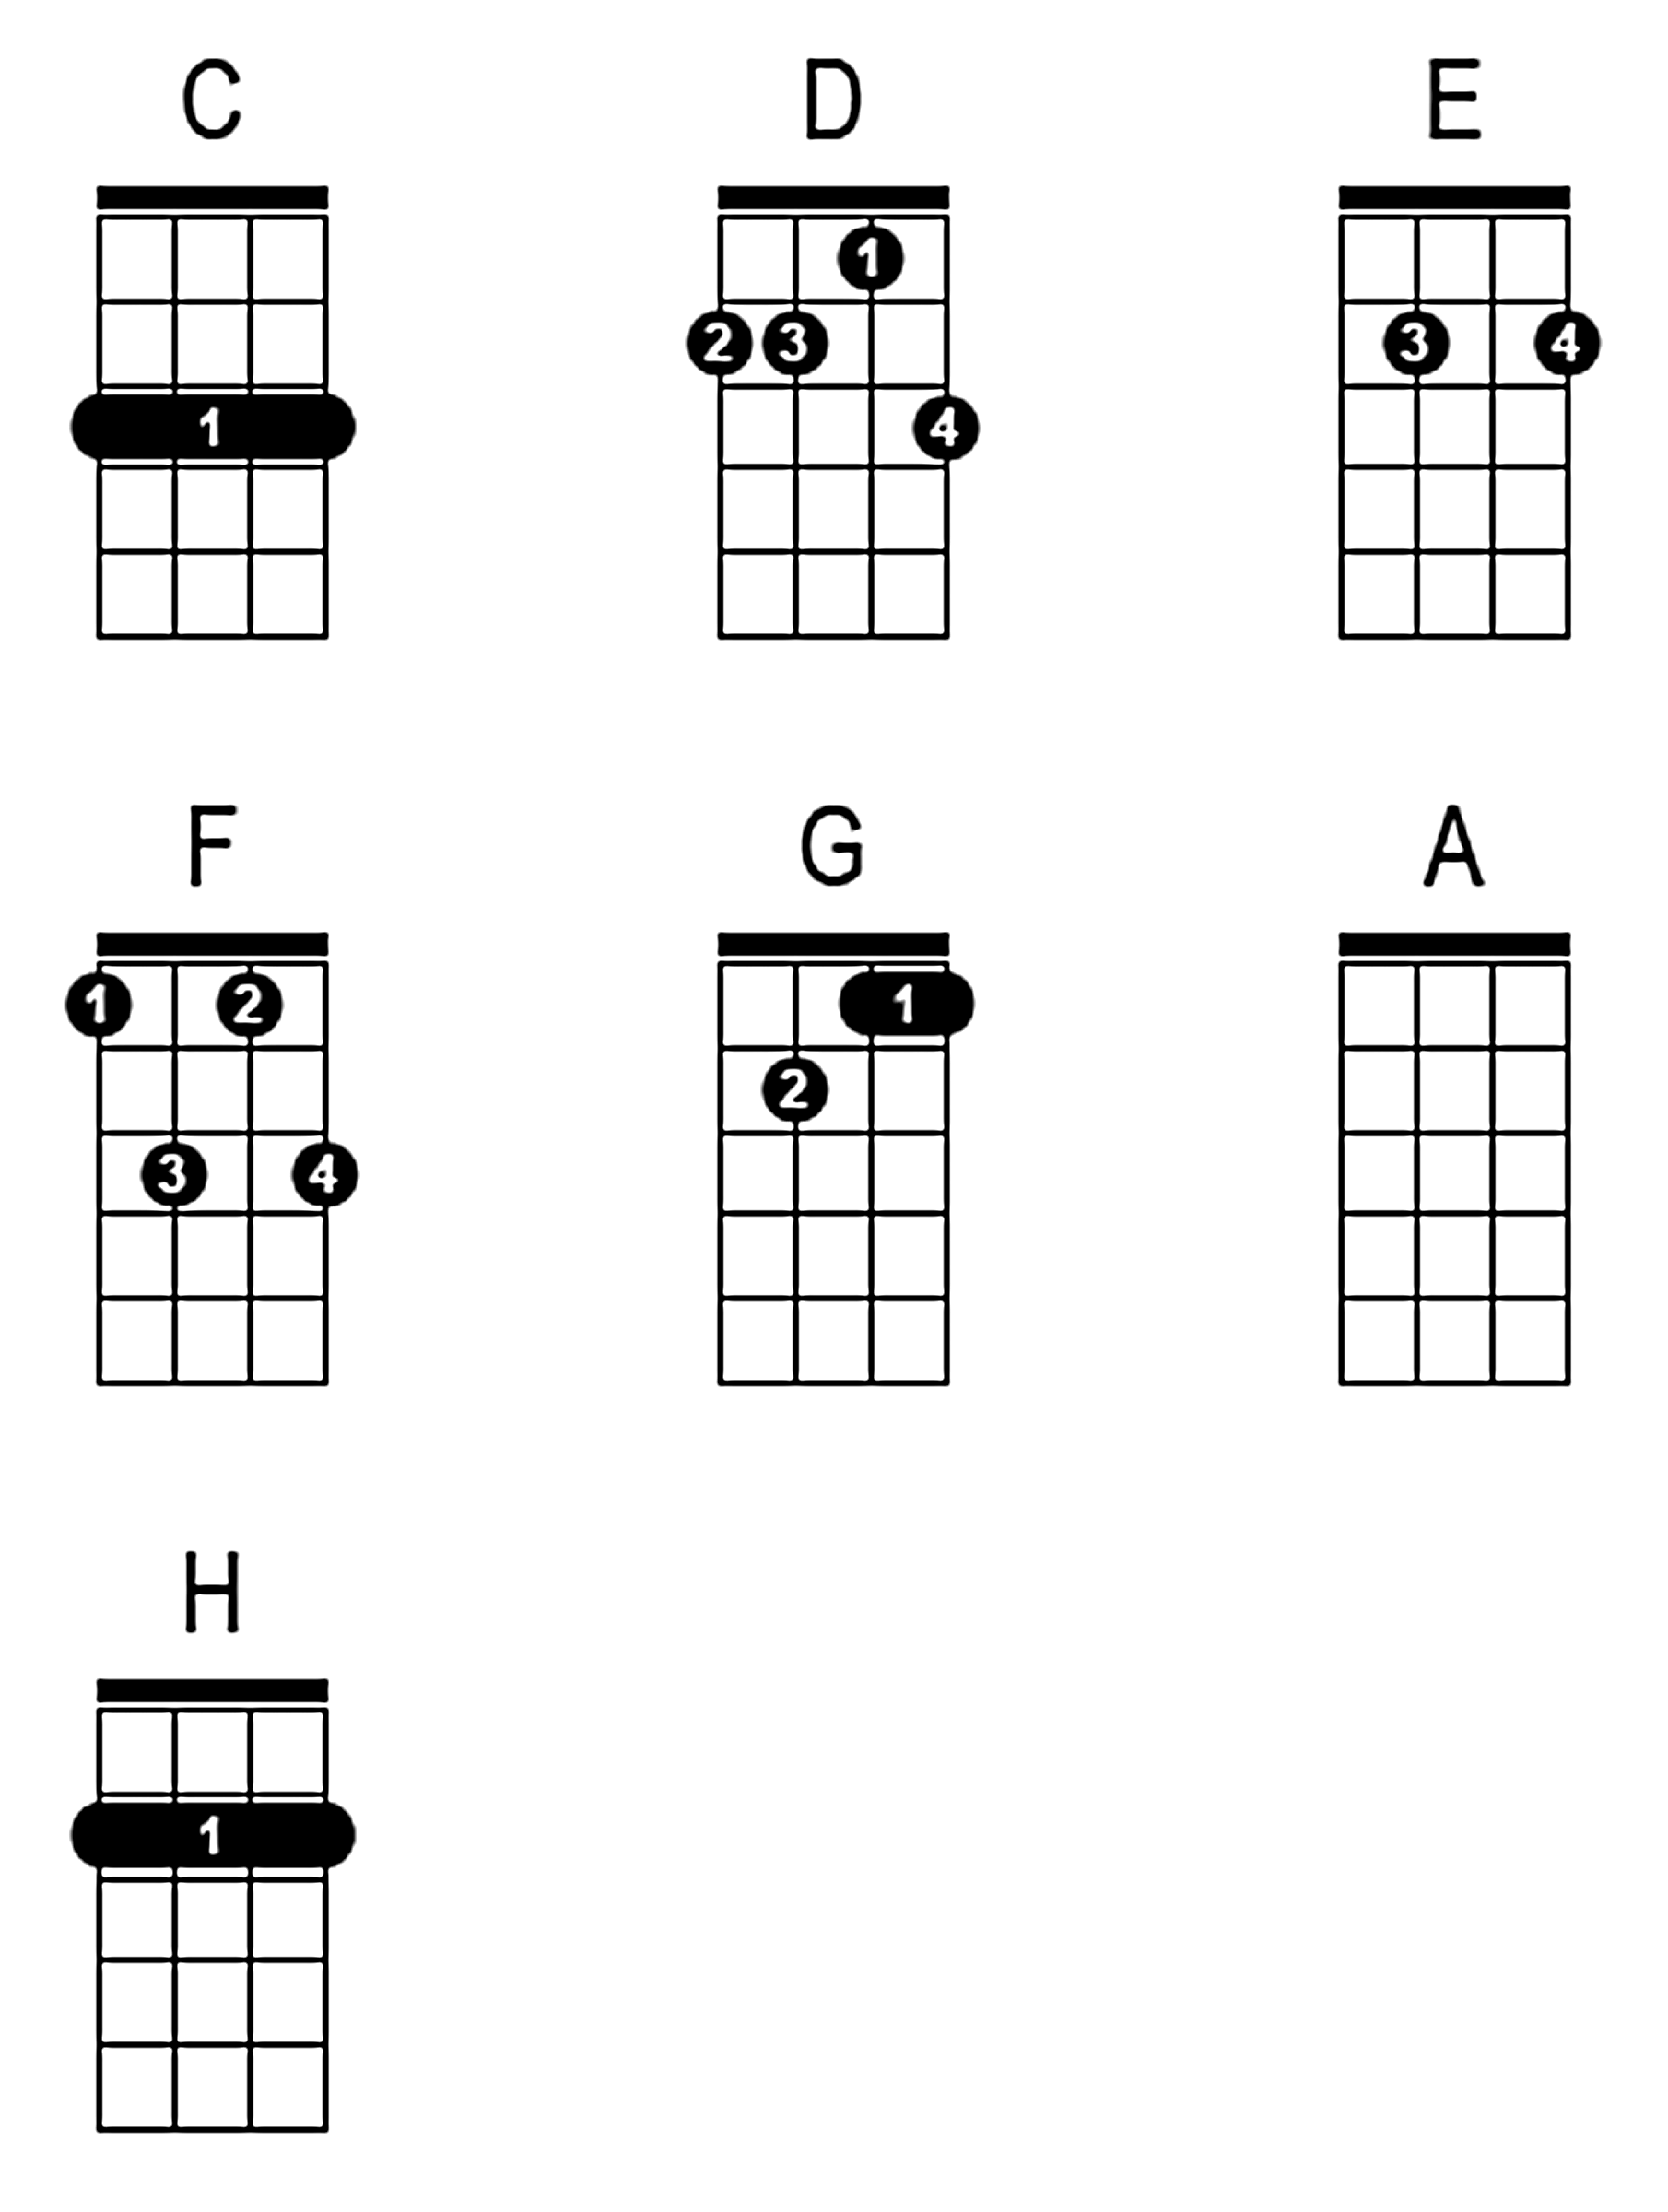
\includegraphics[width=0.25\linewidth]{../images/acc06_m7}
\hfill\\%
%
~\\~\\~\\~\\~\\
%
\makebox[\textwidth][s]{\textit{~sus2 ~ sus4 ~ Maj7 ~ Dim7~}}\\~\\~\\
%
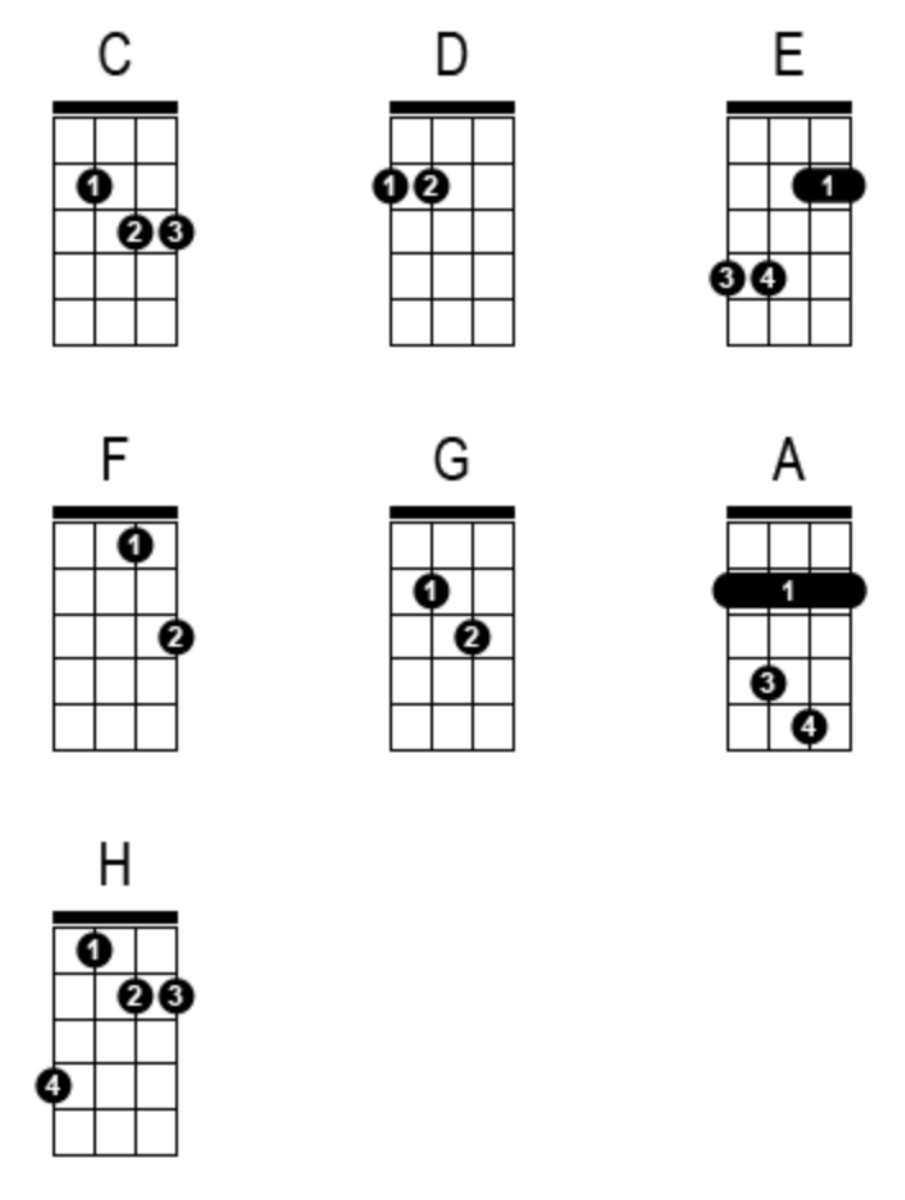
\includegraphics[width=0.2\linewidth]{../images/acc07_sus2}
\hfill
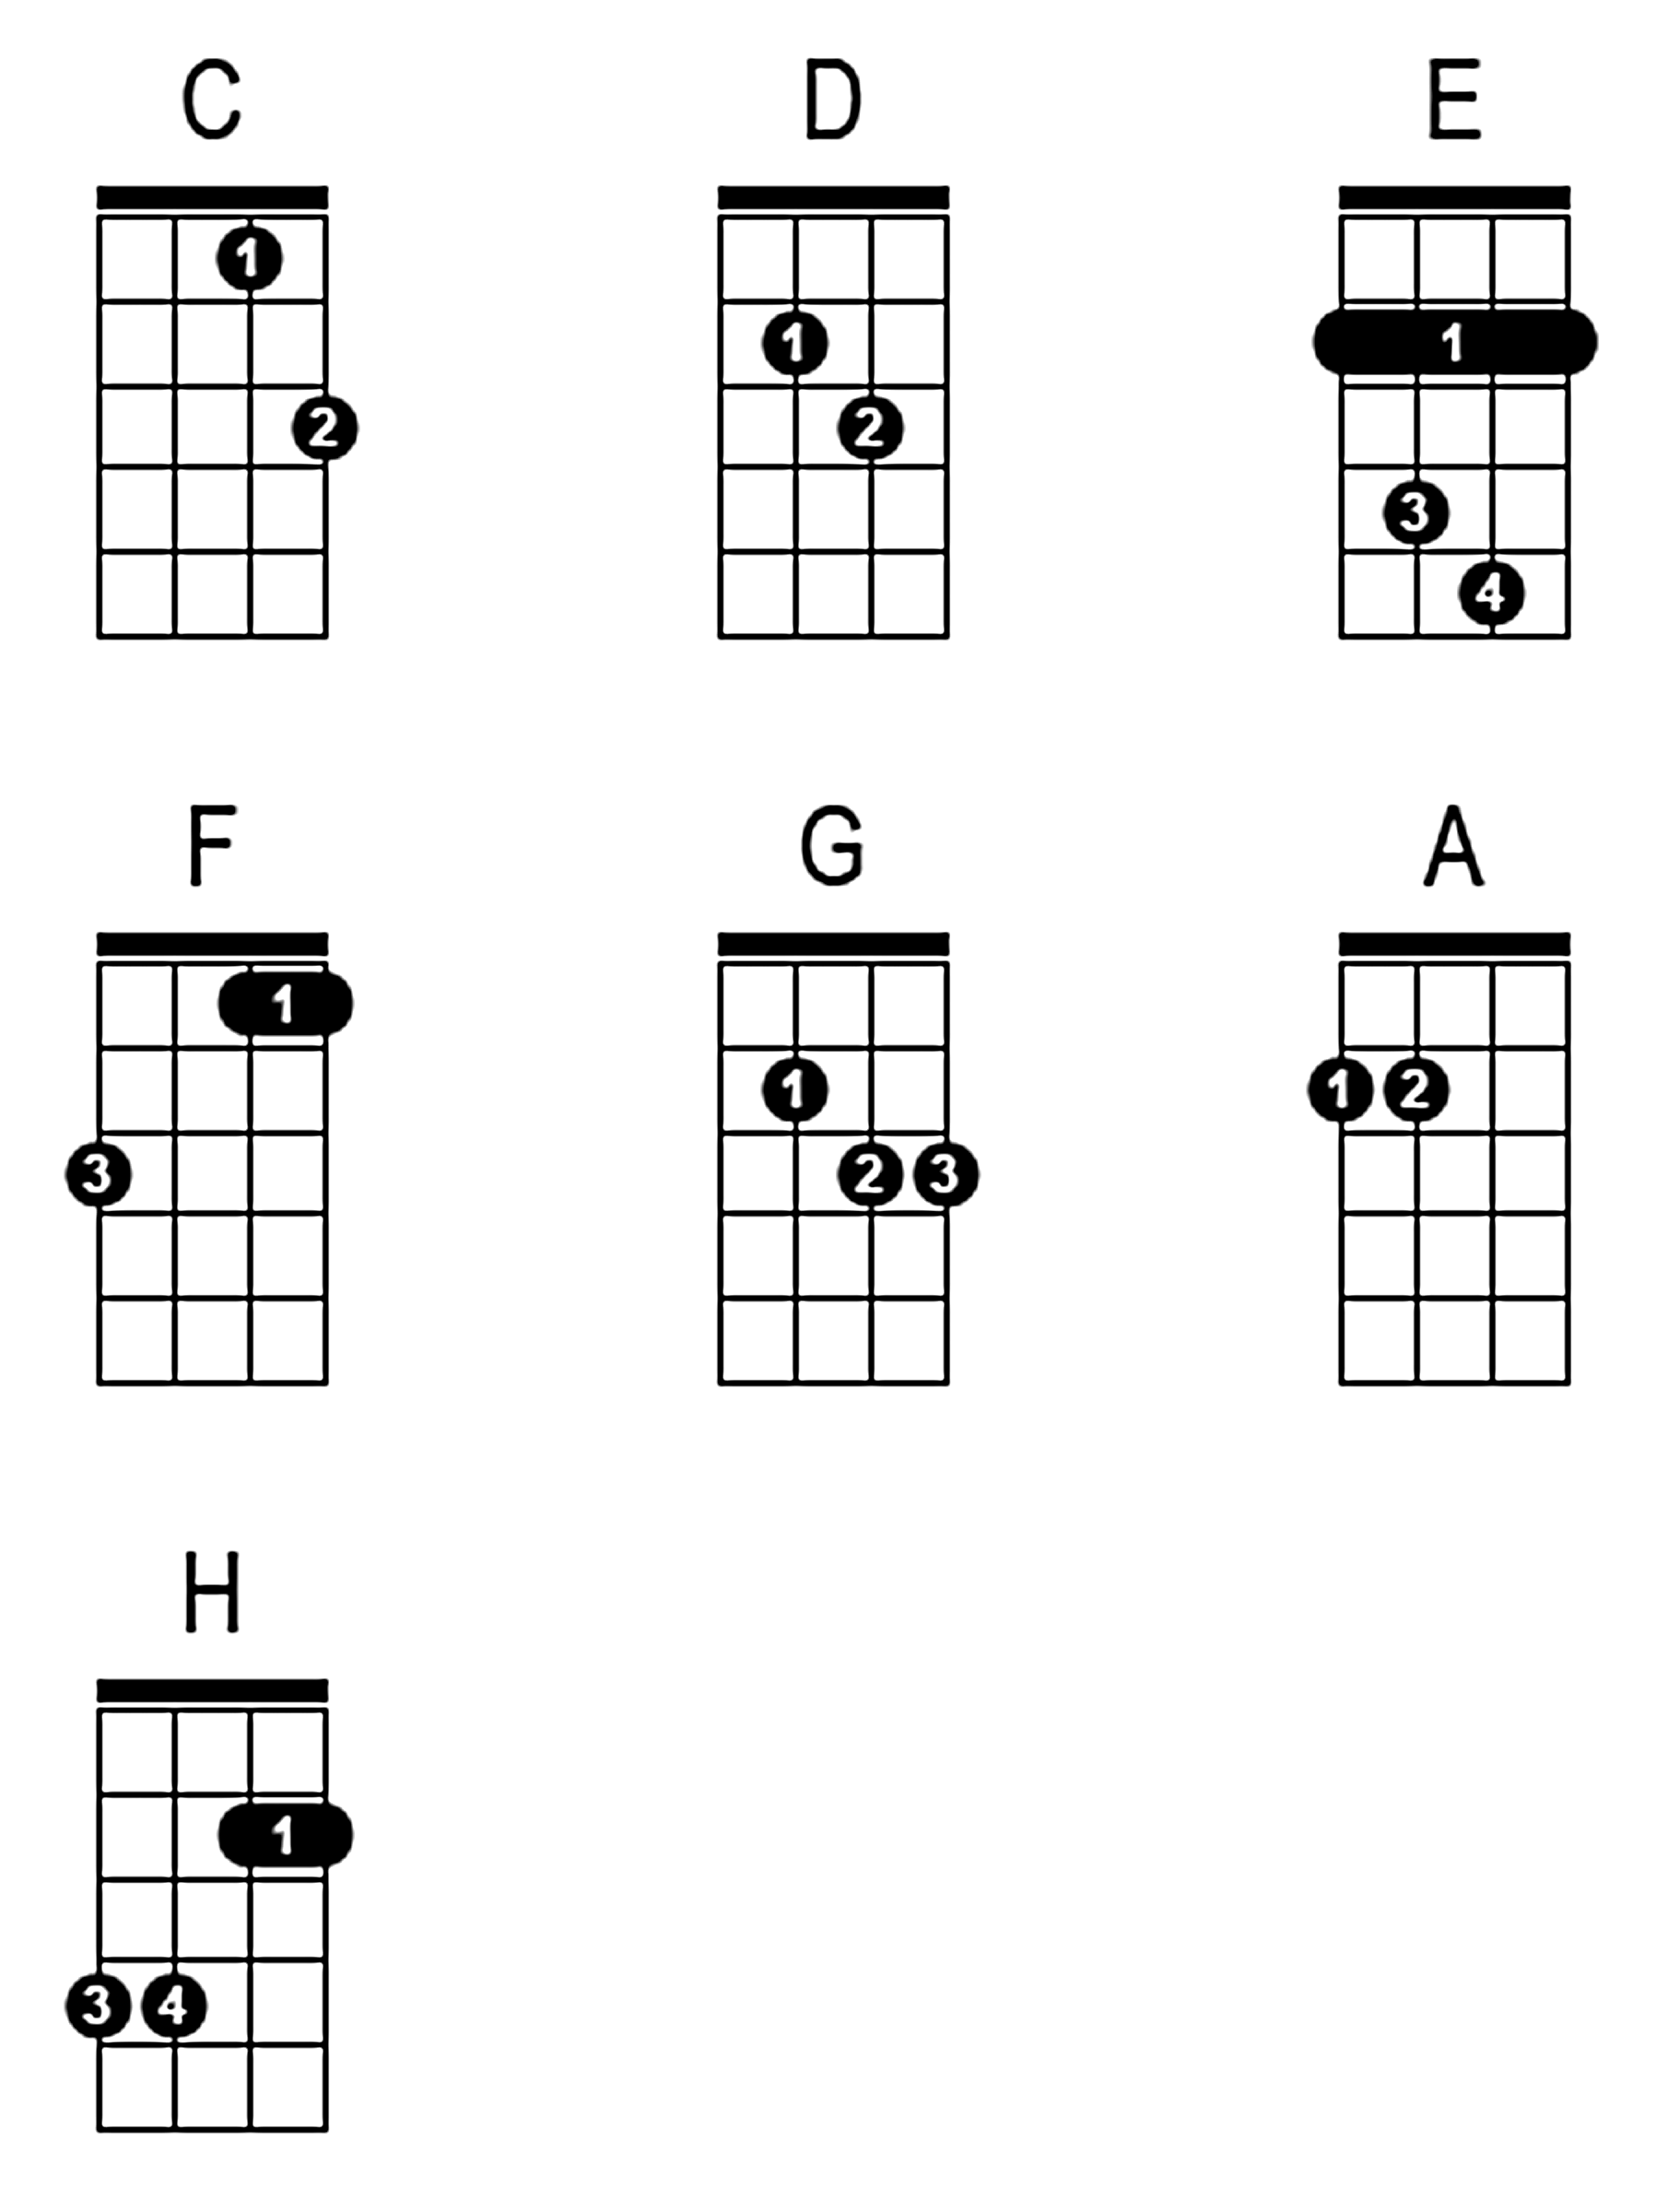
\includegraphics[width=0.2\linewidth]{../images/acc08_sus4}
\hfill
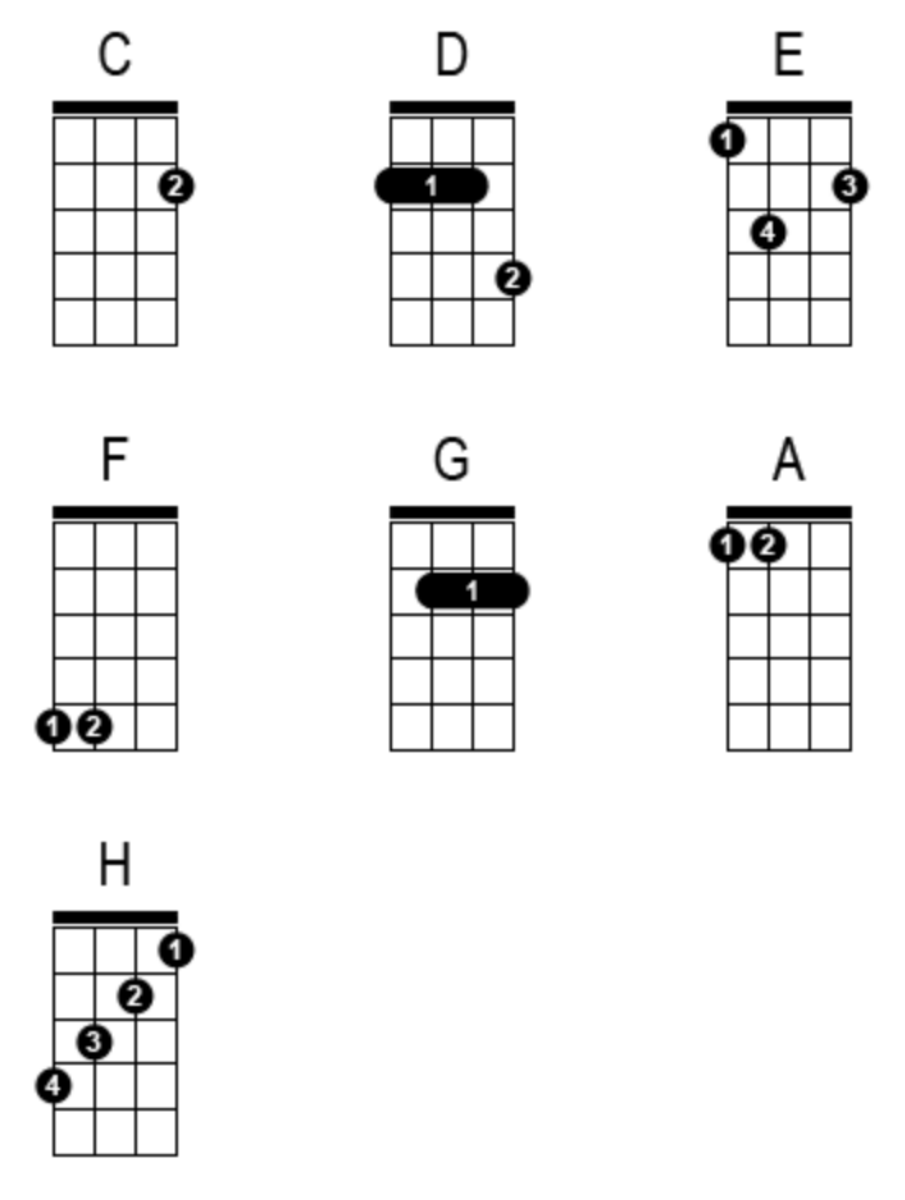
\includegraphics[width=0.2\linewidth]{../images/acc09_Maj7}
\hfill
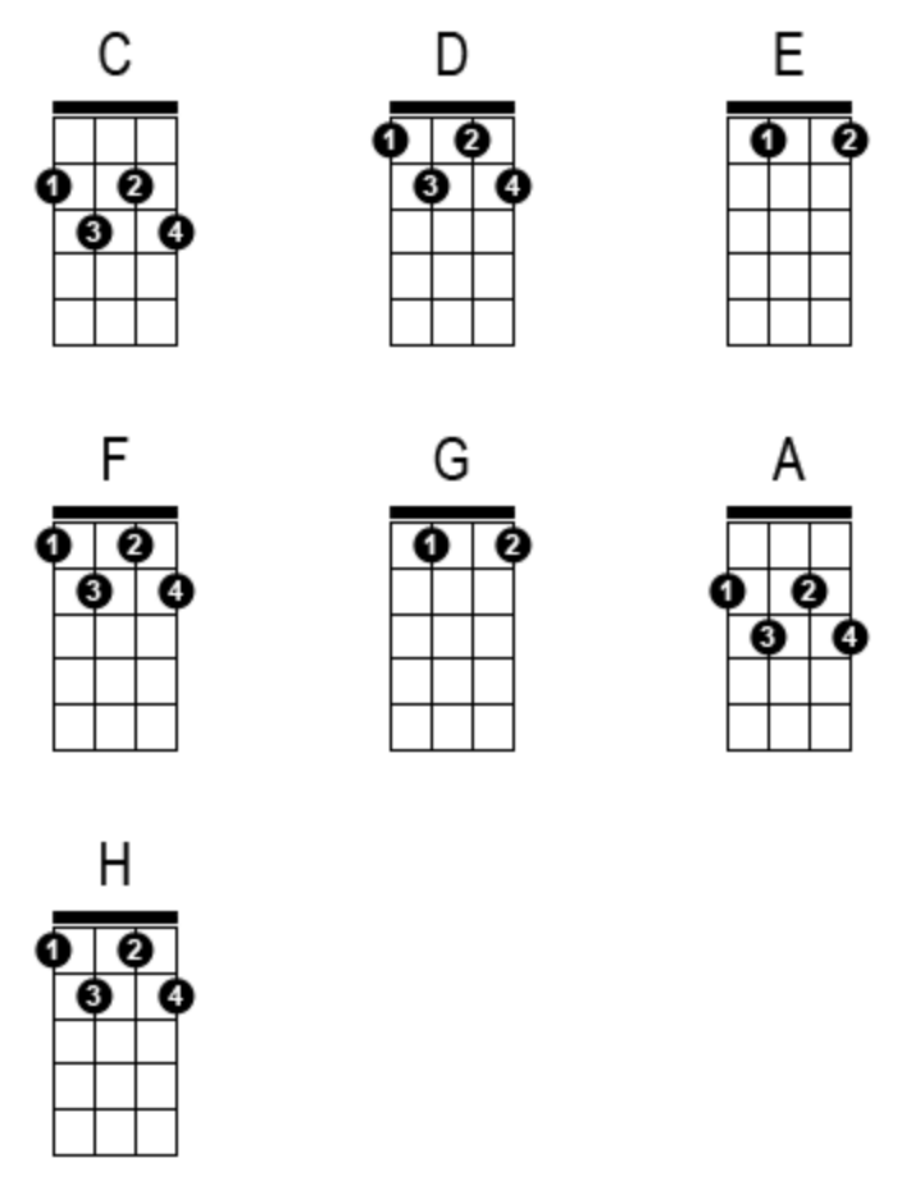
\includegraphics[width=0.2\linewidth]{../images/acc10_Dim7}
%\hfill

\clearpage
%\drawukulelechord{2,1,0,0}
\hspace{-2.2cm}%
\renewcommand{\arraystretch}{3.5}
%  copied from here: https://tex.stackexchange.com/questions/318670/generating-ukulele-chord-diagrams
\begin{tabular}{r|ccccccccccccc}
	         & maj                        & 6                           & 7                           & 9                           & maj7                        & m                           & m6                          & m7                          & m9                          & sus2                        & sus4                        & +                           & dim                         \\\hline
	C        & \drawukulelechord{0,0,0,3} & \drawukulelechord{0,0,0,0} & \drawukulelechord{0,0,0,1} & \drawukulelechord{0,2,0,1} & \drawukulelechord{0,0,0,2} & \drawukulelechord{0,3,3,3} & \drawukulelechord{0,3,3,0} & \drawukulelechord{3,3,3,3} & \drawukulelechord{5,3,3,5} & \drawukulelechord{0,2,3,3} & \drawukulelechord{0,0,1,3} & \drawukulelechord{1,0,0,3} & \drawukulelechord{2,3,2,3} \\
	\shortstack[r]{C\# \\\vspace{-0.5cm}/ Db} & \drawukulelechord{1,1,1,4} & \drawukulelechord{1,1,1,1} & \drawukulelechord{1,1,1,2} & \drawukulelechord{1,3,1,2} & \drawukulelechord{1,1,1,3} & \drawukulelechord{5,3,3,3} & \drawukulelechord{1,4,4,1} & \drawukulelechord{1,4,4,2} & \drawukulelechord{1,3,0,4} & \drawukulelechord{1,3,4,4} & \drawukulelechord{1,1,2,4} & \drawukulelechord{2,1,1,0} & \drawukulelechord{0,1,0,1} \\
	D        & \drawukulelechord{2,2,2,0} & \drawukulelechord{2,2,2,2} & \drawukulelechord{2,2,2,3} & \drawukulelechord{2,4,2,3} & \drawukulelechord{2,2,2,4} & \drawukulelechord{2,2,1,0} & \drawukulelechord{2,2,1,2} & \drawukulelechord{2,2,1,3} & \drawukulelechord{2,4,1,5} & \drawukulelechord{2,2,0,0} & \drawukulelechord{0,2,3,0} & \drawukulelechord{3,2,2,1} & \drawukulelechord{1,2,1,2} \\
	\shortstack[r]{D\# \\\vspace{-0.5cm}/ Eb} & \drawukulelechord{0,3,3,1} & \drawukulelechord{3,3,3,3} & \drawukulelechord{3,3,3,4} & \drawukulelechord{0,1,1,1} & \drawukulelechord{3,3,3,5} & \drawukulelechord{3,3,2,1} & \drawukulelechord{3,0,2,1} & \drawukulelechord{3,1,2,1} & \drawukulelechord{3,5,2,6} & \drawukulelechord{3,3,1,1} & \drawukulelechord{1,3,4,1} & \drawukulelechord{0,3,3,2} & \drawukulelechord{2,3,2,3} \\
	E        & \drawukulelechord{4,4,4,2} & \drawukulelechord{1,1,0,2} & \drawukulelechord{1,2,0,2} & \drawukulelechord{1,2,2,2} & \drawukulelechord{1,3,0,2} & \drawukulelechord{0,4,3,2} & \drawukulelechord{4,4,3,4} & \drawukulelechord{0,2,0,2} & \drawukulelechord{0,4,2,2} & \drawukulelechord{4,4,2,2} & \drawukulelechord{2,4,5,2} & \drawukulelechord{1,0,0,3} & \drawukulelechord{0,1,0,1} \\
	F        & \drawukulelechord{2,0,1,0} & \drawukulelechord{2,2,1,3} & \drawukulelechord{2,3,1,0} & \drawukulelechord{2,3,3,3} & \drawukulelechord{2,4,1,3} & \drawukulelechord{1,0,1,3} & \drawukulelechord{1,2,1,3} & \drawukulelechord{1,3,1,3} & \drawukulelechord{0,5,4,3} & \drawukulelechord{0,0,1,3} & \drawukulelechord{3,0,1,1} & \drawukulelechord{2,1,1,0} & \drawukulelechord{1,2,1,2} \\
	\shortstack[r]{F\# \\\vspace{-0.5cm}/ Gb} & \drawukulelechord{3,1,2,1} & \drawukulelechord{3,3,1,4} & \drawukulelechord{3,4,2,0} & \drawukulelechord{1,1,0,1} & \drawukulelechord{3,5,2,4} & \drawukulelechord{2,1,2,0} & \drawukulelechord{2,3,2,4} & \drawukulelechord{2,4,2,4} & \drawukulelechord{1,1,2,0} & \drawukulelechord{1,1,2,4} & \drawukulelechord{4,2,3,3} & \drawukulelechord{3,2,2,1} & \drawukulelechord{2,3,2,3} \\
	G        & \drawukulelechord{0,2,3,2} & \drawukulelechord{0,2,0,2} & \drawukulelechord{0,2,1,2} & \drawukulelechord{2,2,1,2} & \drawukulelechord{0,2,2,2} & \drawukulelechord{0,2,3,1} & \drawukulelechord{0,2,0,1} & \drawukulelechord{0,2,1,1} & \drawukulelechord{2,2,3,1} & \drawukulelechord{0,2,3,0} & \drawukulelechord{0,2,3,3} & \drawukulelechord{0,3,3,2} & \drawukulelechord{0,1,0,1} \\
	\shortstack[r]{G\# \\\vspace{-0.5cm}/ Ab} & \drawukulelechord{5,3,4,3} & \drawukulelechord{1,3,1,3} & \drawukulelechord{1,3,2,3} & \drawukulelechord{3,3,2,3} & \drawukulelechord{1,3,3,3} & \drawukulelechord{4,3,4,2} & \drawukulelechord{1,3,1,2} & \drawukulelechord{1,3,2,2} & \drawukulelechord{3,3,4,2} & \drawukulelechord{1,3,4,1} & \drawukulelechord{1,3,4,4} & \drawukulelechord{1,0,0,3} & \drawukulelechord{1,2,1,2} \\
	A        & \drawukulelechord{2,1,0,0} & \drawukulelechord{2,1,2,0} & \drawukulelechord{0,1,0,0} & \drawukulelechord{0,1,0,2} & \drawukulelechord{1,1,0,0} & \drawukulelechord{2,0,0,0} & \drawukulelechord{2,0,2,0} & \drawukulelechord{0,0,0,0} & \drawukulelechord{2,0,0,2} & \drawukulelechord{2,4,5,2} & \drawukulelechord{2,2,0,0} & \drawukulelechord{2,1,1,0} & \drawukulelechord{2,3,2,3} \\
	\shortstack[r]{A\# \\\vspace{-0.5cm}/ B}  & \drawukulelechord{3,2,1,1} & \drawukulelechord{0,2,1,1} & \drawukulelechord{1,2,1,1} & \drawukulelechord{1,2,1,3} & \drawukulelechord{3,2,1,0} & \drawukulelechord{3,1,1,1} & \drawukulelechord{3,1,3,1} & \drawukulelechord{1,1,1,1} & \drawukulelechord{3,1,1,3} & \drawukulelechord{3,0,1,1} & \drawukulelechord{3,3,1,1} & \drawukulelechord{3,2,2,1} & \drawukulelechord{0,1,0,1} \\
	H        & \drawukulelechord{4,3,2,2} & \drawukulelechord{1,3,2,2} & \drawukulelechord{2,3,2,2} & \drawukulelechord{2,3,2,4} & \drawukulelechord{4,3,2,1} & \drawukulelechord{4,2,2,2} & \drawukulelechord{1,2,2,2} & \drawukulelechord{2,2,2,2} & \drawukulelechord{4,2,2,4} & \drawukulelechord{4,1,2,2} & \drawukulelechord{4,4,2,2} & \drawukulelechord{0,3,3,2} & \drawukulelechord{1,2,1,2}
\end{tabular}